%
% Copyright 2018 Joel Feldman, Andrew Rechnitzer and Elyse Yeager.
% This work is licensed under a Creative Commons Attribution-NonCommercial-ShareAlike 4.0 International License.
% https://creativecommons.org/licenses/by-nc-sa/4.0/
%
\questionheader{ex:s1.2}

%%%%%%%%%%%%%%%%%%
\subsection*{\Conceptual}
%%%%%%%%%%%%%%%%%%
\begin{question}
For each of the following properties of definite integrals, draw a picture illustrating the concept, interpreting definite integrals as areas under a curve.

For simplicity, you may assume that $a \leq c \leq b$, and that $f(x),g(x)$ give positive values.
\begin{enumerate}[(a)]
\item $\displaystyle\int_a^a f(x)\,\dee{x}=0$\qquad
(Theorem~\eref{CLP101}{thm:Intdomain}.a in the CLP-2 text)
\item $\displaystyle\int_a^b f(x)\,\dee{x}= \displaystyle\int_a^c f(x)\,\dee{x} + \int_c^b f(x)\dee{x} $\qquad (Theorem~\eref{CLP101}{thm:Intdomain}.c in the CLP-2 text)
\item $\displaystyle\int_a^b \left( f(x) + g(x) \right)\,\dee{x}
= \displaystyle\int_a^b f(x)\,\dee{x} + \displaystyle\int_a^b g(x)\,\dee{x}$\qquad (Theorem~\eref{CLP101}{thm:Intarith}.a  in the CLP-2 text)
\end{enumerate}
\end{question}
\begin{hint}
\begin{enumerate}[(a)]
\item What is the length of this figure?
\item Think about cutting the area into two pieces vertically.
\item Think about cutting the area into two pieces another way.
\end{enumerate}
\end{hint}
\begin{answer}
Possible drawings:
\begin{center}
\begin{tikzpicture}
\YEaaxis{1}{2.5}{1}{3}
\YExcoord{1}{a}
\draw[thick] plot[domain=-.5:2] (\x,{\x*\x/2+.25}) node[right] {$y=f(x)$};
\draw[thick, blue] (1,0)--(1,.75);
\end{tikzpicture}
\hfill
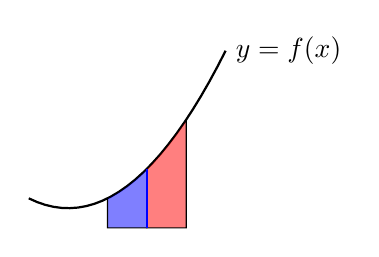
\begin{tikzpicture}
\YEaaxis{1}{2.5}{1}{3}
\YExcoord{.5}{a}
\YExcoord{1}{c}
\YExcoord{1.5}{b}
\draw[thick] plot[domain=-.5:2] (\x,{\x*\x/2+.25}) node[right] {$y=f(x)$};

\draw[fill=blue, fill opacity=0.5] plot[domain=.5:1] (\x,{\x*\x/2+.25})--(1,.75)--(1,0)--(.5,0)--cycle;
\draw[fill=red, fill opacity=0.5] plot[domain=1:1.5] (\x,{\x*\x/2+.25})--(1.5,1.375)--(1.5,0)--(1,0)--cycle;

\draw[thick, blue] (1,0)--(1,.75);
\end{tikzpicture}
\hfill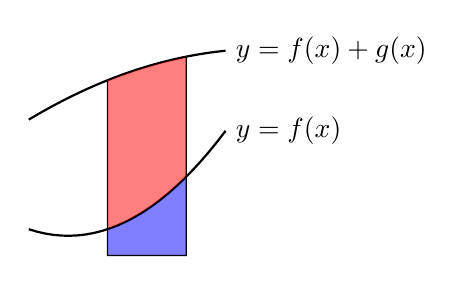
\begin{tikzpicture}
\YEaaxis{1}{2.5}{1}{3}
\YExcoord{.5}{a}
\YExcoord{1.5}{b}
\draw[thick] plot[domain=-.5:2] (\x,{\x*\x/3+.25}) node[right] {$y=f(x)$};
\draw[thick] plot[domain=-.5:2] (\x,{2+\x/2-\x*\x/10}) node[right] {$y=f(x)+g(x)$};
\draw[fill=blue, fill opacity=0.5] plot[domain=.5:1.5] (\x,{\x*\x/3+.25})--(1.5,0)--(.5,0)--cycle;
\draw[fill=red, fill opacity=0.5]plot[domain=.5:1.5] (\x,{2+\x/2-\x*\x/10})--
plot[domain=1.5:.5] (\x,{\x*\x/3+.25}) --cycle;
\end{tikzpicture}
\end{center}

\end{answer}
\begin{solution}
\begin{enumerate}[(a)]
\item $\displaystyle\int_a^a f(x)\,\dee{x}=0$
\begin{center}
\begin{tikzpicture}
\YEaaxis{1}{2.5}{1}{2}
\YExcoord{1}{a}
\draw[thick] plot[domain=-.5:2] (\x,{\x*\x/2+.25}) node[right] {$y=f(x)$};
\draw[thick, blue] (1,0)--(1,.75);
\end{tikzpicture}
\end{center}
The area under the curve is zero, because it's a region with no width.

\item $\displaystyle\int_a^b f(x)\,\dee{x}=\textcolor{blue}{ \displaystyle\int_a^c f(x)\,\dee{x}} +\textcolor{red}{ \int_c^b f(x)\dee{x} }$

\begin{center}
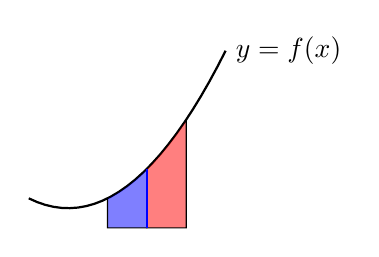
\begin{tikzpicture}
\YEaaxis{1}{2.5}{1}{2}
\YExcoord{.5}{a}
\YExcoord{1}{c}
\YExcoord{1.5}{b}
\draw[thick] plot[domain=-.5:2] (\x,{\x*\x/2+.25}) node[right] {$y=f(x)$};

\draw[fill=blue, fill opacity=0.5] plot[domain=.5:1] (\x,{\x*\x/2+.25})--(1,.75)--(1,0)--(.5,0)--cycle;
\draw[fill=red, fill opacity=0.5] plot[domain=1:1.5] (\x,{\x*\x/2+.25})--(1.5,1.375)--(1.5,0)--(1,0)--cycle;

\draw[thick, blue] (1,0)--(1,.75);
\end{tikzpicture}
\end{center}

If we assume $a \leq c \leq b$, then this identity simply tells us that  if we add up the area under the curve from $a$ to $c$, and from $c$ to $b$, then we get the whole area under the curve from $a$ to $b$.

(The situation is slightly more complicated when $c$ is not between $a$ and $b$, but it still works out.)

\item $\displaystyle\int_a^b \left( f(x) + g(x) \right)\,\dee{x}
=\textcolor{blue}{ \displaystyle\int_a^b f(x)\,\dee{x}} +\textcolor{red}{ \displaystyle\int_a^b g(x)\,\dee{x}}$

\begin{center}
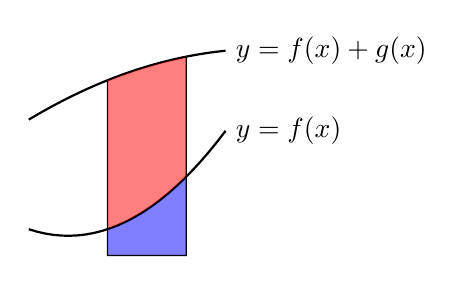
\begin{tikzpicture}
\YEaaxis{1}{2.5}{1}{3}
\YExcoord{.5}{a}
\YExcoord{1.5}{b}
\draw[thick] plot[domain=-.5:2] (\x,{\x*\x/3+.25}) node[right] {$y=f(x)$};
\draw[thick] plot[domain=-.5:2] (\x,{2+\x/2-\x*\x/10}) node[right] {$y=f(x)+g(x)$};
\draw[fill=blue, fill opacity=0.5] plot[domain=.5:1.5] (\x,{\x*\x/3+.25})--(1.5,0)--(.5,0)--cycle;
\draw[fill=red, fill opacity=0.5]plot[domain=.5:1.5] (\x,{2+\x/2-\x*\x/10})--
plot[domain=1.5:.5] (\x,{\x*\x/3+.25}) --cycle;
\end{tikzpicture}
\end{center}

The blue-shaded area in the picture above is $\displaystyle\int_a^b f(x)\ \dee{x}$. The area under the curve $f(x)+g(x)$ but above the curve $f(x)$ (shown in red) is $\displaystyle\int_a^b g(x)\ \dee{x}$.
\end{enumerate}\end{solution}


\begin{Mquestion} If $\displaystyle\int_0^b \cos x\ \dee{x}=\sin b$, then what is $\displaystyle\int_a^b \cos x\
\dee{x}$?
\end{Mquestion}
\begin{hint}
Use the identity $\int\limits_a^b f(x)\ \dee{x} =
\int\limits_a^c f(x)\ \dee{x}+
\int\limits_c^b f(x)\ \dee{x}$.
\end{hint}
\begin{answer}
$\sin b-\sin a$
\end{answer}
\begin{solution}
Using the identity
\begin{align*}
\int\limits_a^b f(x)\ \dee{x} &=
\int\limits_a^c f(x)\ \dee{x}+
\int\limits_c^b f(x)\ \dee{x}\ ,
\intertext{ we see}
\int\limits_a^b\cos x\ \dee{x} &=
\int\limits_a^0 \cos x\ \dee{x}+
\int\limits_0^b \cos x\ \dee{x}\\&=
-\int\limits_0^a \cos x\ \dee{x}+
\int\limits_0^b \cos x\ \dee{x}\\
&=-\sin a + \sin b\\
&=\sin b - \sin a
\end{align*}
\end{solution}

\begin{Mquestion}[2015A, 2016A]
Decide whether each of the following statements is true or false.
If false, provide a counterexample. If true, provide a brief justification.

\begin{enumerate}[(a)]
\item
$\displaystyle\int_{-3}^{-2} f(x) \dee{x}=-\displaystyle\int_{3}^{2} f(x) \dee{x}$.
\item
If $f(x)$ is an odd function, then $\displaystyle \int_{-3}^{-2} f(x)\,\dee{x} = \int_2^3 f(x)\,\dee{x}$.
\item
$\displaystyle\int_{0}^{1} f(x)\cdot g(x) ~\dee{x}
   =\int_{0}^{1} f(x) ~\dee{x} \cdot \int_{0}^{1} g(x) ~\dee{x}$.
\end{enumerate}
\end{Mquestion}

%\begin{hint}
%\end{hint}

\begin{answer}
(a) False. For example, the function
\begin{align*}
f(x) = \begin{cases}
               0 & \text{for $x<0$} \\
               1 & \text{for $x\ge0$}
      \end{cases}
\end{align*}
provides a counterexample.

\noindent (b)
False. For example, the function $f(x)=x$ provides a counterexample.

\noindent (c)
False. For example, the functions
\begin{align*}
f(x) = \begin{cases}
               0 & \text{for $x<\frac{1}{2}$} \\
               1 & \text{for $x\ge\frac{1}{2}$}
      \end{cases}
&&\mbox{and}&&g(x) = \begin{cases}
               0 & \text{for $x\ge \frac{1}{2}$} \\
               1 & \text{for $x<\frac{1}{2}$}
      \end{cases}
\end{align*}
provide a counterexample.


\end{answer}

\begin{solution} (a)
False. For example if
\begin{align*}
f(x) = \begin{cases}
               0 & \text{for $x<0$} \\
               1 & \text{for $x\ge0$}
      \end{cases}
\end{align*}
then \textcolor{blue}{$\int_{-3}^{-2} f(x) \dee{x}=0$} and \textcolor{red}{$-\int_{3}^{2} f(x) \dee{x}=\int^{3}_{2} f(x) \dee{x}=1$}.

\begin{center}
\begin{tikzpicture}
\YEaaxis{2.5}{2.5}{.5}{1.25}
\draw[thick] (-2.25,0)--(0,0) node[opendot]{};
\draw[thick] (0,1)node[vertex]{}--(2.25,1) ;
\YExcoord{-2}{-3}
\YExcoord{-1.33}{-2}
\YExcoord{2}{3}
\YExcoord{1.33}{2}
\draw[ultra thick, blue] (-2,0)--(-1.33,0);
\draw[red, thick, fill=red, fill opacity=0.5] (1.33,0) rectangle (2,1);
\end{tikzpicture}
\end{center}

\noindent (b)
False.  For example, if $f(x)=x$, then \textcolor{blue}{$\int_{-3}^{-2} f(x)\,\dee{x} $} is negative while
\textcolor{red}{$\int_2^3 f(x)\,\dee{x} $} is positive, so they cannot be the same.


\begin{center}
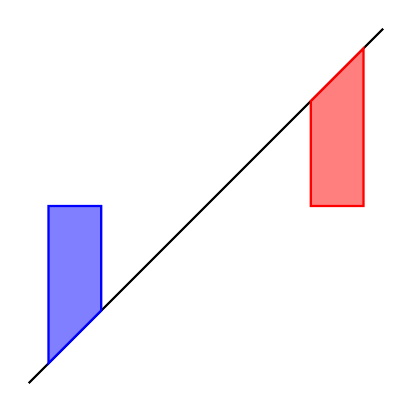
\begin{tikzpicture}
\YEaxis{2.5}{2.5}
\draw[thick] (-2.25,-2.25)--(2.25,2.25);
\YEnxcoord{-2}{-3}
\YEnxcoord{-1.33}{-2}
\YExcoord{2}{3}
\YExcoord{1.33}{2}
\draw[thick, blue, fill=blue, fill opacity=0.5] (-2,-2)--(-1.33,-1.33)|-(-2,0)--cycle;
\draw[red, thick, fill=red, fill opacity=0.5] (1.33,1.33) --(2,2)|-(1.33,0)--cycle;
\end{tikzpicture}
\end{center}


\noindent (c)
False.  For example, consider the functions
\begin{align*}
f(x) = \begin{cases}
               0 & \text{for $x<\frac{1}{2}$} \\
               1 & \text{for $x\ge\frac{1}{2}$}
      \end{cases}
&&\mbox{and}&&g(x) = \begin{cases}
               0 & \text{for $x\ge \frac{1}{2}$} \\
               1 & \text{for $x<\frac{1}{2}$}
      \end{cases}
\end{align*}

Then $f(x)\cdot g(x)=0$ for all $x$, so $\int_0^1 f(x)\cdot g(x) \dee{x}=0$. However,
\textcolor{blue}{$\int_0^1 f(x) \dee{x}= \frac{1}{2}$} and \textcolor{red}{$\int_0^1 g(x) \dee{x}= \frac{1}{2}$}, so $\int_0^1 f(x)\dee{x} \cdot \int_0^1 g(x) \dee{x}= \frac{1}{4}$.

\begin{center}
\begin{tikzpicture}
\YExcoord{1}{\frac{1}{2}}
\YExcoord{2}{1}
\YEycoord{1}{1}
\YEaaxis{.5}{2.5}{.5}{1.25}
\draw[blue, fill=blue, fill opacity=0.5] (1,1)rectangle (2,0);
\draw[thick] (-.25,0)--(1,0) node[opendot]{};
\draw[thick] (1,1)node[vertex]{}--(2.25,1)  node[right]{$f(x)$};
\end{tikzpicture}
\hspace{2cm}
\begin{tikzpicture}
\YExcoord{1}{\frac{1}{2}}
\YExcoord{2}{1}
\YEycoord{1}{1}
\YEaaxis{.5}{2.5}{.5}{1.25}
\draw[red, fill=red, fill opacity=0.5] (0,1)rectangle (1,0);
\draw[thick] (1,0)node[vertex]{}--(2.25,0)  node[above]{$g(x)$};
\draw[thick] (-.25,1)--(1,1) node[opendot]{};
\end{tikzpicture}
\end{center}

\end{solution}
%%%%%%%%%%%%%%%%%%%


\begin{question}
Suppose we want to make a right Riemann sum with 100 intervals to approximate $\int\limits_5^0 f(x)\ \dee{x}$, where $f(x)$ is a function that gives only positive values.\\[5pt]
\begin{enumerate}[(a)]
\item What is $\Delta x$?
\item Are the heights of our rectangles positive or negative?
\item Is our Riemann sum positive or negative?
\item Is the signed area under the curve $y=f(x)$ from $x=0$ to $x=5$ positive or negative?
\end{enumerate}
\end{question}
\begin{hint}
Note that the limits of the integral given are in the opposite order from what we might expect: the smaller number is the top limit of integration.

Recall $\De x = \frac{b-a}{n}$.
\end{hint}
\begin{answer}
(a) $-\dfrac{1}{20}$
\qquad
(b) positive
\qquad
(c) negative
\qquad
(d) positive

\end{answer}
\begin{solution}
\begin{enumerate}[(a)]
\item $\Delta x = \dfrac{b-a}{n}=\dfrac{0-5}{100} = -\dfrac{1}{20}$

Note: if we were to use the Riemann-sum definition of a definite integral, this is how we would justify the identity $\int\limits_a^b f(x)\dee{x}=-\int\limits_b^a f(x)\dee{x}$.

\item The heights of the rectangles are given by $f(x_i)$, where $x_i = a+i\Delta x = 5 - \frac{i}{20}$. Since $f(x)$ only gives positive values, $f(x_i) >0$, so the heights of the rectangles are positive.

\item Our Riemann sum is the sum of the signed areas of individual rectangles. Each rectangle has a negative base ($\Delta x$) and a positive height ($f(x_i)$).  So, each term of our sum is negative. If we add up negative numbers, the sum is negative. So, the Riemann sum is negative.
\item Since $f(x)$ is always above the $x$-axis, $\int\limits_0^5 f(x)\dee{x}$ is positive.
\end{enumerate}

\end{solution}


%%%%%%%%%%%%%%%%%%
\subsection*{\Procedural}
%%%%%%%%%%%%%%%%%%

\begin{question}[M105 2015A]
Suppose $\displaystyle\int_2^3 f(x)\,\dee{x} = -1$ and
$\displaystyle\int_2^3 g(x)\,\dee{x} = 5$. Evaluate
$\displaystyle \int_2^3 \big( 6 f(x) - 3 g(x) \big)\,\dee{x}$.
\end{question}

\begin{hint}
Split the ``target integral'' up into pieces that can be evaluated using the given integrals.
\end{hint}

\begin{answer}
$-21$
\end{answer}

\begin{solution}
The operation of integration is linear (that's
part (d) of the ``arithmetic of integration''
Theorem  \eref{CLP101}{thm:Intarith} in the CLP-2 text),
so that:
\begin{align*}
\int_2^3 [6 f(x) -3 g(x)]\,\dee{x}
&= \int_2^3 6 f(x)\,\dee{x}  - \int_2^3 3 g(x)\,\dee{x} \\
&= 6 \int_2^3  f(x)\,\dee{x}  - 3\int_2^3 g(x)\,\dee{x}
= (6 \times (-1)) - (3 \times 5)
= -21
\end{align*}

\end{solution}


\begin{question}[2016Q1]
If $\displaystyle\int_0^2 f(x)\,\dee{x} = 3$ and
$\displaystyle\int_0^2 g(x)\,\dee{x} = -4$, calculate
$\displaystyle \int_0^2 \big( 2 f(x) + 3 g(x) \big)\,\dee{x}$.
\end{question}

\begin{hint}
Split the ``target integral'' up into pieces that can be evaluated using the given integrals.
\end{hint}

\begin{answer}
$-6$
\end{answer}

\begin{solution}
The operation of integration is linear (that's
part (d) of the ``arithmetic of integration''
Theorem  \eref{CLP101}{thm:Intarith} in the CLP-2 text),
so that:
\begin{align*}
\int_0^2 [2 f(x) +3 g(x)]\,\dee{x}
   &= \int_0^2 2 f(x)\,\dee{x}  + \int_0^2 3 g(x)\,\dee{x} \\
&= 2 \int_0^2  f(x)\,\dee{x}  + 3\int_0^2 g(x)\,\dee{x} = (2 \times 3) + (3 \times (-4)) = -6
\end{align*}

\end{solution}


\begin{Mquestion}[2016Q1]
 The functions $f(x)$ and $g(x)$ obey
\begin{equation*}
\int_0^{-1} f(x)\,\dee{x} = 1 \qquad
\int_0^2 f(x)\,\dee{x} = 2 \qquad
\int_{-1}^0 g(x)\,\dee{x} = 3 \qquad
\int_0^2 g(x)\,\dee{x} = 4
\end{equation*}
Find $\int_{-1}^2 \big[3g(x)-f(x)\big]\,\dee{x}$.
\end{Mquestion}

\begin{hint}
Split the ``target integral'' up into pieces that can be evaluated using the given integrals.
\end{hint}

\begin{answer}
20
\end{answer}

\begin{solution}
Using part (d) of the ``arithmetic of integration'' Theorem  \eref{CLP101}{thm:Intarith},
followed by parts (c) and (b) of the ``arithmetic for the domain of integration'' Theorem
  \eref{CLP101}{thm:Intdomain} in the
%\href{http://www.math.ubc.ca/%7Efeldman/m101/clp/clp_notes_101.pdf}{CLP 101 notes}.
 in the CLP-2 text,
\begin{align*}
\int_{-1}^2 \big[3g(x)-f(x)\big]\,\dee{x}
&=3\int_{-1}^2 g(x)\,\dee{x}-\int_{-1}^2 f(x)\,\dee{x} \\
&=3\int_{-1}^0 g(x)\,\dee{x}+3\int_0^2 g(x)\,\dee{x}
-\int_{-1}^0 f(x)\,\dee{x}-\int_0^2 f(x)\,\dee{x} \\
&=3\int^0_{-1} g(x)\,\dee{x}+3\int_0^2 g(x)\,\dee{x}
+\int_0^{-1} f(x)\,\dee{x}-\int_0^2 f(x)\,\dee{x} \\
&=3\times 3+3\times 4 + 1 - 2 = 20
\end{align*}

\end{solution}
%%%%%%%%%%%%%%%%%%%%%%%%
\begin{question} In Question~\ref{1.1_awkwardcircle}, Section 1.1, we found that
\[\int_0^a\sqrt{1-x^2}\ \dee{x}=\frac{\pi}{4} - \frac{1}{2}\arccos(a)+\frac{1}{2}a\sqrt{1-a^2}\]
when $0\le a\le 1$.

Using this fact, evaluate the following:
\begin{enumerate}[(a)]
\item $\displaystyle\int_{a}^0 \sqrt{1-x^2}\ \dee{x}$, where $-1 \leq a \leq 0$
\item $\displaystyle\int_{a}^1 \sqrt{1-x^2}\ \dee{x}$, where $0 \leq a \leq 1$
\end{enumerate}
\end{question}
\begin{hint} For part (a), use the symmetry of the integrand. For part (b), the area $\int	\limits_{0}^1 \sqrt{1-x^2}\ \dee{x}$ is easy to find--how is this useful to you?
\end{hint}
\begin{answer}
\begin{enumerate}[(a)]
\item $\frac{\pi}{4} - \frac{1}{2}\arccos(-a)-\frac{1}{2}a\sqrt{1-a^2}
=-\frac{\pi}{4} + \frac{1}{2}\arccos(a)-\frac{1}{2}a\sqrt{1-a^2}$
\item $\frac{1}{2}\arccos(a)-\frac{1}{2}a\sqrt{1-a^2}$
\end{enumerate}
\end{answer}
\begin{solution}
\begin{enumerate}[(a)]
\item Since $\sqrt{1-x^2}$ is an even function,
\begin{align*}
\int_{a}^0 \sqrt{1-x^2}\ \dee{x} 
&=\int_{0}^{|a|} \sqrt{1-x^2}\ \dee{x}  = \frac{\pi}{4} - \frac{1}{2}\arccos(|a|)+\frac{1}{2}|a|\sqrt{1-|a|^2}\\
&=\frac{\pi}{4} - \frac{1}{2}\arccos(-a)-\frac{1}{2}a\sqrt{1-a^2}
\end{align*}
Alternatively, since $\arccos(-a) = \pi-\arccos(a)$ we also have
\begin{align*}
\int_{a}^0 \sqrt{1-x^2}\ \dee{x} 
&=-\frac{\pi}{4} + \frac{1}{2}\arccos(a)-\frac{1}{2}a\sqrt{1-a^2}
\end{align*}

\item Note $\displaystyle\int_{0}^1 \sqrt{1-x^2}\ \dee{x}=\frac{\pi}{4}$, since the area under the curve represents one-quarter of the unit circle. Then,
\begin{align*}\displaystyle\int_{a}^1 \sqrt{1-x^2}\ \dee{x}&=
\displaystyle\int_{0}^1 \sqrt{1-x^2}\ \dee{x}-
\displaystyle\int_{0}^a \sqrt{1-x^2}\ \dee{x}\\
&=\frac{\pi}{4}-\left(\frac{\pi}{4} - \frac{1}{2}\arccos(a)+\frac{1}{2}a\sqrt{1-a^2}\right)\\
&=\frac{1}{2}\arccos(a)-\frac{1}{2}a\sqrt{1-a^2}
\end{align*}
\end{enumerate}

\end{solution}


%%%%%%%%%%%%%%%%%%%%%%%%

\begin{Mquestion}[M105 2013A]\label{prob:s1.2_2}
Evaluate ${\displaystyle\int_{-1}^2 |2x|\ \dee{x}}$.

You may use the result from  Example \eref{CLP101}{eg:INTPROPx}  in the CLP-2 text
that
$
\int\limits_a^b x\ \dee{x}=\frac{b^2-a^2}{2}
$.

\end{Mquestion}

\begin{hint}
The evaluation of this integral was also the subject of Question
\ref{prob:s1.2_2} in Section 1.1. This time try using the method
of Example \eref{CLP101}{eg:INTPROPabs} in the
%\href{http://www.math.ubc.ca/%7Efeldman/m101/clp/clp_notes_101.pdf}{CLP 101 notes}.
CLP-2 text.
\end{hint}

\begin{answer}
$5$
\end{answer}

\begin{solution}
Recall that
\begin{align*}
|x|=\begin{cases} -x &\text{if $x\le 0$}\\
                   x &\text{if $x\ge 0$}
    \end{cases}
\end{align*}
so that
\begin{align*}
|2x|=\begin{cases} -2x &\text{if $x\le 0$}\\
                    2x &\text{if $x\ge 0$}
    \end{cases}
\end{align*}
Also recall, from  Example \eref{CLP101}{eg:INTPROPx} in the
%\href{http://www.math.ubc.ca/%7Efeldman/m101/clp/clp_notes_101.pdf}{CLP 101 notes}.
CLP-2 text that
\begin{align*}
\int_a^b x\ \dee{x}&=\frac{b^2-a^2}{2}
\end{align*}
So
\begin{align*}
\int_{-1}^2 |2x|\ \dee{x}
&=\int_{-1}^0 |2x|\ \dee{x}+\int_0^2 |2x|\ \dee{x}
=\int_{-1}^0 (-2x)\ \dee{x}+\int_0^2 2x\ \dee{x} \\
&= -2\int_{-1}^0 x\ \dee{x}+2\int_0^2 x\ \dee{x}
=-2\cdot\frac{0^2-(-1)^2}{2} +2\cdot\frac{2^2-0^2}{2} \\
&=1+4=5
\end{align*}


\end{solution}
%%%%%%%%%%%%%%%%%%%



\begin{question}
Evaluate $\displaystyle\int_{-5}^5 x|x|\ \dee{x}$\,.
\end{question}
\begin{hint} Use symmetry.
\end{hint}
\begin{answer} 0
\end{answer}
\begin{solution}
We note that the integrand $f(x)=x|x|$ is an odd function, because $f(-x)=-x|-x|=-x|x|=-f(x)$. Then, by Theorem~\eref{CLP101}{thm:INTevenodd}.b in the CLP-2 text,
 $\displaystyle\int_{-5}^5 x|x| \ \dee{x}=0$.
\end{solution}

\begin{Mquestion}
Suppose $f(x)$ is an even function and $\displaystyle\int_{-2}^2 f(x)\dee{x}=10$. What is
$\displaystyle\int_{-2}^0 f(x)\dee{x}$?
\end{Mquestion}
\begin{hint}
Check Theorem~\eref{CLP101}{thm:INTevenodd} in the CLP-2 text.
\end{hint}
\begin{answer} 5
\end{answer}
\begin{solution}
Using Theorem~\eref{CLP101}{thm:INTevenodd}.a in the CLP-2 text,
\begin{align*}10&=\int_{-2}^2 f(x)\dee{x}=2\int_{0}^2f(x)\dee{x}\\
5&=\int_{0}^2f(x)\dee{x}
\intertext{Also,}
\int_{-2}^2 f(x)\dee{x}&=\int_{-2}^0 f(x)\dee{x}+\int_{0}^2 f(x)\dee{x}
\intertext{So,}
\int_{-2}^0 f(x)\dee{x}&=\int_{-2}^2 f(x)\dee{x}-\int_{0}^2 f(x)\dee{x}\\
&=10-5=5
\end{align*}
Indeed, for any even function $f(x)$, $\int\limits_{-a}^0 f(x)\dee{x} = \int\limits_{0}^a f(x)\dee{x}$.
\end{solution}

%%%%%%%%%%%%%%%%%%
\subsection*{\Application}
%%%%%%%%%%%%%%%%%%

\begin{question}[2016Q1]
Evaluate $\displaystyle\int_{-2}^{2} \left(5+\sqrt{4-x^2}\right)\dee{x}$.
\end{question}

\begin{hint}
Split the integral into a sum of two integrals. Interpret each geometrically.
\end{hint}

\begin{answer}
$20 +2\pi$
\end{answer}

\begin{solution}
We first use additivity:
\begin{align*}
 \int_{-2}^{2} \left(5+\sqrt{4-x^2}\right)\dee{x} =
\textcolor{blue}{  \int_{-2}^{2} 5\,\dee{x} }+ \textcolor{red}{\int_{-2}^{2} \sqrt{4-x^2}\,\dee{x}}
\end{align*}
The first integral represents the area of a rectangle of height 5 and width 4 and so equals $20$.
The second integral represents the area above the $x$--axis and below the curve $y=\sqrt{4-x^2}$ or $x^2+y^2=4$. That is a semicircle of radius 2, which has area
$\frac{1}{2}\pi 2^2$. So
\begin{align*}
 \int_{-2}^{2} \left(5+\sqrt{4-x^2}\right)\dee{x} =
\textcolor{blue}{20} +\textcolor{red}{2\pi}
\end{align*}

\begin{center}
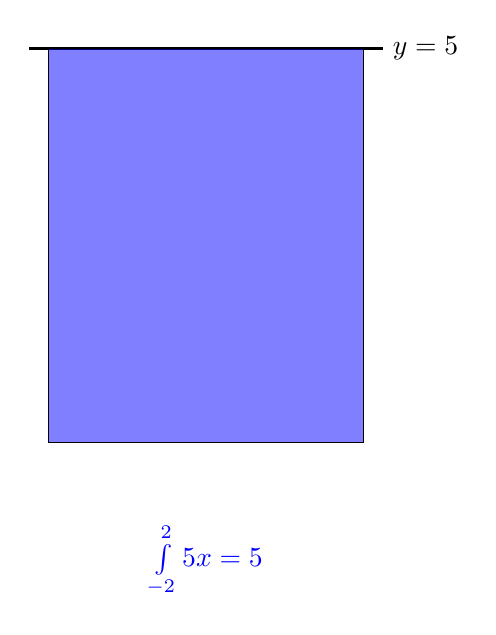
\begin{tikzpicture}
\YEaaxis{2.5}{2.5}{.5}{5.5}
\YExcoord{2}{2}
\YExcoord{-2}{-2}
\draw[thick] (-2.25,5)--(2.25,5);
\draw[fill=blue, fill opacity=0.5] (-2,0) rectangle (2,5);
\draw (2.25,5) node[right]{$y=5$};
\draw[blue] (0,-1.5) node{$\int\limits_{-2}^2 5 \dee{x}=5$};
\end{tikzpicture}
\hspace{2cm}
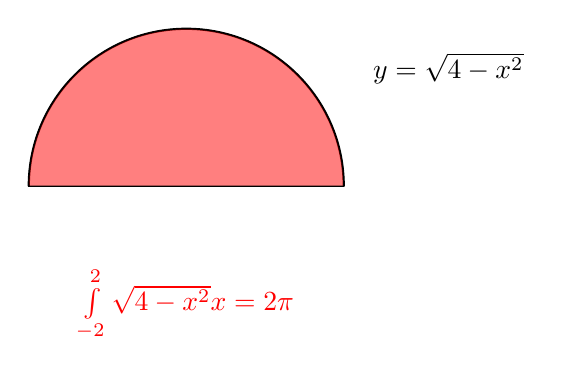
\begin{tikzpicture}
\YEaaxis{2.5}{2.5}{.5}{5.5}
\draw[thick] (-2,0) arc (180:0:2cm);
\YExcoord{2}{2}
\YExcoord{-2}{-2}
\draw[fill=red, fill opacity=0.5] (-2,0) arc (180:0:2cm)--cycle;
\draw (2.25,1.5) node[right]{$y=\sqrt{4-x^2}$};
\draw[red] (0,-1.5) node{$\int\limits_{-2}^2 \sqrt{4-x^2} \dee{x}=2\pi$};
\end{tikzpicture}
\end{center}
\end{solution}
%%%%%%%%%%%%%%%%%%%



\begin{Mquestion}[M121 2012A]
Evaluate $\displaystyle\int_{-2012}^{+2012} \frac{\sin x}{\log(3+x^2)}\dee{x}$.
\end{Mquestion}

\begin{hint}
Hmmmm.  Looks like a complicated integral. It's probably a trick question.
Check for symmetries.
\end{hint}

\begin{answer}
$0$
\end{answer}

\begin{solution}
Note that the integrand $f(x) = \frac{\sin x}{\log(3+x^2)}$ is an odd function, because:
\begin{equation*}
f(-x) = \frac{\sin(-x)}{\log(3+(-x)^2)}=\frac{-\sin x}{\log(3+x^2)} =- f(x)
\end{equation*}
The domain of integration $-2012 \le x \le 2012$ is symmetric about $x=0$. So,
by Theorem \eref{CLP101}{thm:INTevenodd} of the CLP-2 text,
\begin{equation*}
\int_{-2012}^{+2012} \frac{\sin x}{\log(3+x^2)}\dee{x} = 0
\end{equation*}
\end{solution}
%%%%%%%%%%%%%%%%%%%

\begin{question}[2012A]
Evaluate $\displaystyle\int_{-2012}^{+2012} x^{1/3}\cos x\,\dee{x}$.
\end{question}

\begin{hint}
Check for symmetries again.
\end{hint}

\begin{answer}
$0$
\end{answer}

\begin{solution}
Note that the integrand $f(x) = x^{1/3}\cos x$ is an odd function,
because:
\begin{equation*}
f(-x) = (-x)^{1/3}\cos(-x)= - x^{1/3}\cos x =- f(x)
\end{equation*}
The domain of integration $-2012 \le x \le 2012$ is symmetric about $x=0$. So,
by Theorem \eref{CLP101}{thm:INTevenodd} of the CLP-2 text,
\begin{equation*}
\int_{-2012}^{+2012}x^{1/3}\cos x\,\dee{x} = 0
\end{equation*}
\end{solution}
%%%%%%%%%%%%%%%%%%%

\begin{question}
Evaluate $\displaystyle\int_{0}^6 (x-3)^3\,\dee{x}$\,.
\end{question}
\begin{hint}
What does the integrand look like to the left and right of $x=3$?
\end{hint}
\begin{answer}
0
\end{answer}
\begin{solution}
Our integrand $f(x)=(x-3)^3$ is neither even nor odd. However, it does have a similar symmetry. Namely, $f(3+x)=-f(3-x)$. So, $f$ is ``negatively symmetric" across the line $x=3$. This suggests that the integral should be 0: the positive area to the right of $x=3$ will be the same as the negative area to the left of $x=3$.

Another way to see this is to notice that the graph of $f(x)=(x-3)^3$ is equivalent to the graph of $g(x)=x^3$ shifted three units to the right, and $g(x)$ is an odd function. So,
\[\textcolor{red}{\int_{0}^6 (x-3)^3\,\dee{x}} = \textcolor{blue}{\int_{-3}^3 x^3\,\dee{x}}=0\]

\begin{center}
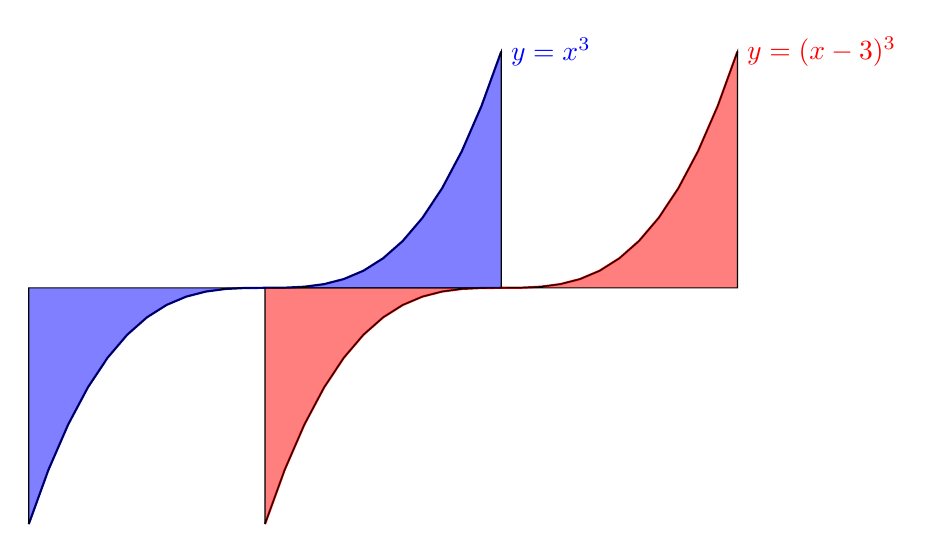
\begin{tikzpicture}
\YEaaxis{3.5}{6.5}{3.5}{3}
\foreach \x in {-3,3,6}{\YExcoord{\x}{\x}}
\draw[thick, blue] plot[domain=-3:3] (\x,{\x*\x*\x/9});
\draw[blue] (3,3) node[right]{$y=x^3$};
\draw[thick, red] plot[domain=0:6] (\x,{(\x-3)*(\x-3)*(\x-3)/9});
\draw[red] (6,3) node[right]{$y=(x-3)^3$};

\draw[fill=red, fill opacity=0.5] plot[domain=0:6] (\x,{(\x-3)*(\x-3)*(\x-3)/9})|-(3,0)-|(0,-3);
\draw[fill=blue, fill opacity=0.5] plot[domain=-3:3] (\x,{\x*\x*\x/9})|-(0,0)-|(-3,-3);
\end{tikzpicture}
\end{center}
\end{solution}
%%%%%%%%%%%%%%%%%%%


\begin{question}\label{prob_s1.2:ellipsearea}
We want to compute the area of an ellipse, $(ax)^2+(by)^2=1$ for some (let's say positive) constants $a$ and $b$.
\begin{enumerate}[(a)]
\item Solve the equation for the upper half of the ellipse. It should have the form ``$y=\cdots$"
\item Write an integral for the area of the upper half of the ellipse. Using properties of integrals, make the integrand look like the upper half of a circle.
\item Using geometry and your answer to part (b), find the area of the ellipse.
\end{enumerate}
\end{question}
\begin{hint}
In part (b), you'll have to factor a constant out through a square root. Remember the upper half of a circle looks like $\sqrt{r^2-x^2}$.
\end{hint}
\begin{answer}
(a) $y = \dfrac{1}{b}\sqrt{1-(ax)^2}$\qquad
(b) $\displaystyle\frac{a}{b}\int_{-\frac{1}{a}}^{\frac{1}{a}}\sqrt{\frac{1}{a^2}-x^2}\ \dee{x}$
\qquad (c) $\dfrac{\pi}{ab}$
\end{answer}
\begin{solution}
\begin{enumerate}[(a)]
\item
\begin{align*}
(ax)^2+(by)^2&=1\\
by&=\sqrt{1-(ax)^2}\\
y &= \frac{1}{b}\sqrt{1-(ax)^2}
\end{align*}
\item The values of $x$ in the domain of the function above are those that satisfy $1-(ax)^2 \geq 0$. That is, $-\frac{1}{a}\leq x \leq \frac{1}{a}$. Therefore, the upper half of the ellipse has area
\begin{align*}
\displaystyle\frac{1}{b}&\displaystyle\int_{-\frac{1}{a}}^{\frac{1}{a}}\sqrt{1-(ax)^2}\ \dee{x}
\intertext{The upper half of a circle has equation $y=\sqrt{r^2-x^2}$.
}
&=\frac{1}{b}\int_{-\frac{1}{a}}^{\frac{1}{a}}\sqrt{a^2\left(\frac{1}{a^2}-x^2\right)}\ \dee{x}\\
&=\frac{1}{b}\int_{-\frac{1}{a}}^{\frac{1}{a}}a\sqrt{\frac{1}{a^2}-x^2}\ \dee{x}\\
&=\frac{a}{b}\int_{-\frac{1}{a}}^{\frac{1}{a}}\sqrt{\frac{1}{a^2}-x^2}\ \dee{x}
\end{align*}


\item The function $y=\sqrt{\dfrac{1}{a^2}-x^2}$ is the upper-half of the circle centred at the origin with radius $\dfrac{1}{a}$. So, the expression from (b) evaluates to $\left(\dfrac{a}{b}\right)\dfrac{\pi}{2a^2} = \dfrac{\pi}{2ab}$.

The expression from (b) was half of the ellipse, so the area of the ellipse is $\dfrac{\pi}{ab}$.

\end{enumerate}

Remark: this was a slightly long-winded way of getting the result. The reasoning is basically this:
\begin{itemize}
\item The area of the unit circle $x^2+y^2=1$ is $\pi $\ .
\item The ellipse $(ax)^2+y^2=1$ is obtained by shrinking the unit circle horizontally by a factor of $a$. So, its area is $\dfrac{\pi}{a}$\ .
\item Further, the ellipse $(ax)^2+(by)^2=1$ is obtained from the previous ellipse by shrinking it vertically by a factor of $b$. So, its area is $\dfrac{\pi}{ab}$\ .
\end{itemize}
\end{solution}
%%%%%%%%%%%%%%%%%%%

\begin{Mquestion}

Fill in the following table: the product of an (even/odd) function with an (even/odd) function is an (even/odd) function. You may assume that both functions are defined for all real numbers.

\begin{center}
\begin{tabular}{|c||c|c|}
\hline
$\times$&even&odd\\
\hline\hline
even&&\\
\hline
odd&&\\
\hline
\end{tabular}\end{center}
\end{Mquestion}
\begin{hint}
For two functions $f(x)$ and $g(x)$, define $h(x)=f(x)\cdot g(x)$. If $h(-x)=h(x)$, then the product is even; if $h(-x)=-h(x)$, then the product is odd.

The table will \emph{not} be  the same as if we were multiplying even and odd \emph{numbers}.
\end{hint}
\begin{answer}

\begin{tabular}{|c||c|c|}
\hline
$\times$&even&odd\\
\hline\hline
even&even&odd\\
\hline
odd&odd&even\\
\hline
\end{tabular}

\end{answer}
\begin{solution}
Let's recall the definitions of even and odd functions: $f(x)$ is \emph{even} if $f(-x)=f(x)$ for every $x$ in its domain, and $f(x)$ is \emph{odd} if $f(-x)=-f(x)$ for every $x$ in its domain.

Let $h(x)=f(x)\cdot g(x)$.
\begin{description}
\item[even $\times$ even: ] If $f$ and $g$ are both even, then $h(-x)=f(-x)\cdot g(-x) = f(x)\cdot g(x)=h(x)$, so their product is even.
\item[odd $\times$ odd: ] If $f$ and $g$ are both odd, then $h(-x)=f(-x)\cdot g(-x) =[- f(x)]\cdot [-g(x)]=f(x)\cdot g(x)=h(x)$, so their product is even.
\item[even $\times$ odd: ] If $f$ is even and $g$ is odd, then $h(-x)=f(-x)\cdot g(-x) = f(x)\cdot[- g(x)]=-[f(x)\cdot g(x)]=-h(x)$, so their product is odd. Because multiplication is commutative, the order we multiply the functions in doesn't matter.
\end{description}

We note that the table would be the same as if we were \emph{adding} (not multiplying) even and odd \emph{numbers} (not functions).
\end{solution}

%%%%%%%%%%%%%%%%%%%

\begin{question}
Suppose $f(x)$ is an odd function and $g(x)$ is an even function, both defined at $x=0$. What are the possible values of $f(0)$ and $g(0)$?
\end{question}
\begin{hint}
Note $f(0)=f(-0)$.
\end{hint}
\begin{answer}
$f(0)=0$; $g(0)$ can be any real number
\end{answer}
\begin{solution}
Since $f(x)$ is odd, $f(0)=-f(-0)=-f(0)$. So, $f(0)=0$.

However, this restriction does not apply to $g(x)$. For example, for any constant $c$, let $g(x)=c$. Then $g(x)$ is even and $g(0)=c$. So, $g(0)$ can be any real number.
\end{solution}


\begin{question}\label{1.1_bothevenodd}
Suppose $f(x)$ is a function defined on all real numbers that is both even and odd. What could $f(x)$ be?
\end{question}
\begin{hint}
If $f(x)$ is even and odd, then $f(x)=-f(x)$ for every $x$.
\end{hint}
\begin{answer}
$f(x)=0$ for every $x$
\end{answer}
\begin{solution}
Let $x$ be any real number.
\begin{itemize}
\item $f(x)=f(-x)$ (since $f(x)$ is even), and
\item $f(x)=-f(-x)$ (since $f(x)$ is odd).
\item So, $f(x)=-f(x)$.
\item Then (adding $f(x)$ to both sides) we see $2f(x)=0$, so $f(x)=0$.
\end{itemize}
So, $f(x)=0$ for every $x$.
\end{solution}


%%%%%%%%%%%%%%%%%%%%


\begin{Mquestion}\label{1.2_derivevenodd}
Is the derivative of an even function even or odd? Is the derivative of an odd function even or odd?
\end{Mquestion}
\begin{hint}
Think about mirroring a function across an axis. What does this do to the slope?
\end{hint}
\begin{answer}
The derivative of an even function is odd, and the derivative of an odd function is even.
\end{answer}
\begin{solution}

\begin{description}
\item[Solution 1:] Suppose $f(x)$ is an odd function. We investigate $f'(x)$ using the chain rule:
\begin{alignat*}{3}
f(-x)&=-f(x)& \mbox{(odd function)}\\
\diff{}{x}\{f(-x)\}&=\diff{}{x}\{-f(x)\}\\
-f'(-x)&=-f'(x) & \mbox{(chain rule)}\\
f'(-x)&=f'(x)
\end{alignat*}

So, when $f(x)$ is odd, $f'(x)$ is even.

Similarly, suppose $f(x)$ is even.

\begin{alignat*}{3}
f(-x)&=f(x)& \mbox{(even function)}\\
\diff{}{x}\{f(-x)\}&=\diff{}{x}\{f(x)\}\\
-f'(-x)&=f'(x) & \mbox{(chain rule)}\\
f'(-x)&=-f'(x)
\end{alignat*}

So, when $f(x)$ is even,  $f'(x)$ is odd.


\item[Solution 2:]
Another way to think about this problem is to notice that ``mirroring" a function changes the sign of its derivative. Then since an even function is ``mirrored once" (across the $y$-axis), it should have $f'(x)=-f'(-x)$, and so the derivative of an even function should be an odd function. Since an odd function is ``mirrored twice" (across the $y$-axis and across the $x$-axis), it should have $f'(x)=-(-f'(-x))=f'(-x)$. So the derivative of an odd function should be even.
These ideas are presented in more detail below.

First, we consider the case where $f(x)$ is even, and investigate $f'(x)$.
\begin{center}
\begin{tikzpicture}
\YEaxis{5}{3}
\draw[thick,blue] plot[domain=-5:5, samples=50](\x,{2*cos(\x*3.14/5 r)});
\draw[blue] (5,-2) node[right]{$y=f(x)$};
\foreach \x/\y in {1/1,2/2.5,3/4}
{\YExcoord{\y}{a_{\x}}
\YExcoord{-\y}{-a_{\x}}}
\foreach \x/\y in {1/1.6,2.5/0,4/-1.6}{
	\draw[red] (\x,\y) node[vertex]{};
	\draw[red] (-\x,\y) node[vertex]{};}
\foreach \a/\b/\x/\y in {1/1.6/0.5/-0.37,
2.5/0/.5/-0.63,
4/-1.6/.5/-.37}{
\ADD{\a}{\x}{\xx}
\ADD{\b}{\y}{\yy}
\SUBTRACT{\a}{\x}{\xxx}
\SUBTRACT{\b}{\y}{\yyy}
\ADD{-\a}{-\x}{\ww}
\ADD{\b}{\y}{\zz}
\SUBTRACT{-\a}{-\x}{\www}
\SUBTRACT{\b}{\y}{\zzz}
\draw[red, ultra thick] (\xx,\yy)--(\xxx,\yyy);
\draw[red, ultra thick] (\ww,\zz)--(\www,\zzz);}
\end{tikzpicture}
\end{center}

The whole function has a mirror-like symmetry across the $y$-axis. So, at $x$ and $-x$, the function will have the same ``steepness," but if one is increasing then the other is decreasing. That is, $f'(-x)=-f'(x)$. (In the picture above, compare the slope at some point $a_i$ with its corresponding point $-a_i$.) So, $f'(x)$ is odd when $f(x)$ is even.

Second, let's consider the case where $f(x)$ is odd, and investigate $f'(x)$. Suppose the blue graph below is $y=f(x)$. If $f(x)$ were \emph{even}, then to the left of the $y$-axis, it would look like the orange graph, which we'll call $y=g(x)$.

\begin{center}
\begin{tikzpicture}
\YEaxis{5}{3}
\draw[thick,blue] plot[domain=-1.25:1.25, xscale=4, yscale=3, samples=50](\x,{\x*(\x*\x-1)});
\draw[thick,orange, dashed] plot[domain=0:1.25, xscale=4, yscale=3, samples=50](-\x,{\x*(\x*\x-1)});
\draw[orange] (-5,2) node[left]{$y=g(x)$};
\draw[blue] (5,2) node[right]{$y=f(x)$};
\end{tikzpicture}
\end{center}

From our work above, we know that, for every $x>0$, $-f'(x)=g'(-x)$. When $x<0$, $f(x)=-g(x)$. So, if $x>0$, then $-f'(x)=g'(-x)=-f'(-x)$. In other words, $f'(x)=f'(-x)$. Similarly, if $x<0$, then $f'(x)=-g'(x)=f'(-x)$. Therefore $f'(x)$ is even. (In the graph below, you can anecdotally verify that $f'(a_i)=f'(-a_i)$.)

\begin{center}
\begin{tikzpicture}
\YEaxis{5}{3}
\draw[thick,blue] plot[domain=-1.25:1.25, xscale=4, yscale=3, samples=50](\x,{\x*(\x*\x-1)});
\draw[thick,orange, dashed] plot[domain=0:1.25, xscale=4, yscale=3, samples=50](-\x,{\x*(\x*\x-1)});
\draw[orange] (-5,2) node[left]{$y=g(x)$};
\draw[blue] (5,2) node[right]{$y=f(x)$};
\foreach \x/\y in {1/1,2/2.5,3/4}
{\YExcoord{\y}{a_{\x}}
\YExcoord{-\y}{-a_{\x}}}
\foreach \x/\y in {1/-.7,2.5/-1.14,4/0}{
	\draw[red] (\x,\y) node[vertex]{};
	\draw[red] (-\x,-\y) node[vertex]{};
	\draw[orange] (-\x,\y) node[vertex]{};}
\foreach \a/\b/\x/\y in {1/-0.7/0.5/-0.3,
2.5/-1.14/.5/.05,
4/0/.25/.4}{
\ADD{\a}{\x}{\xx}
\ADD{\b}{\y}{\yy}
\SUBTRACT{\a}{\x}{\xxx}
\SUBTRACT{\b}{\y}{\yyy}
\ADD{-\a}{\x}{\ww}
\ADD{-\b}{\y}{\zz}
\SUBTRACT{-\a}{\x}{\www}
\SUBTRACT{-\b}{\y}{\zzz}
\draw[red, ultra thick] (\xx,\yy)--(\xxx,\yyy);
\draw[orange, thick] (-\xx,\yy)--(-\xxx,\yyy);
\draw[red, ultra thick] (\ww,\zz)--(\www,\zzz);}
\end{tikzpicture}
\end{center}
\end{description}

\end{solution}
